\documentclass[12pt, a4paper, oneside]{Thesis} % Paper size, default font size and one-sided paper
\usepackage{wrapfig}
\usepackage{lscape}
\usepackage{rotating}
\usepackage{graphicx}
\usepackage{caption}
\usepackage{amsmath}


\usepackage{lineno,hyperref}
\modulolinenumbers[5]


\usepackage{amssymb}
\usepackage{graphicx}
\usepackage{array}
\usepackage{float}
\usepackage{placeins}
\usepackage{stackengine}
\usepackage{url}
\usepackage{numprint}
\usepackage{caption}

\usepackage{booktabs}  
\usepackage{siunitx}
%\usepackage[showframe=false]{geometry}
\usepackage{subfigure}

\nprounddigits{3}
\newcolumntype{P}[1]{>{\centering\arraybackslash}p{#1}}
\newcolumntype{M}[1]{>{\centering\arraybackslash}m{#1}}

\setstackEOL{\#}
\setstackgap{L}{12pt}


%\usepackage{subcaption} %incompatible with subfig
\graphicspath{{Pictures/}} % Specifies the directory where pictures are stored
\usepackage{natbib} % Use the natbib reference package - read up on this to edit the reference style; if you want text (e.g. Smith et al., 2012) for the in-text references (instead of numbers), remove 'numbers' v

\hypersetup{urlcolor=black, colorlinks=false} % Colors hyperlinks in blue - change to black if annoyingv`	

\thesistitle{Detection of Forest Area in SAR images}
\supervisor{Dr. Jayanta Mukhopadhyay}
\degree{Master of Technology}
\degreemajor{Computer Science \& Engineering}
\authors{Jeffrey Jose}
\rollno{17CS60R77}
\university{Indian Institute of Technology Kharagpur}
\department{Department of Computer Science \& Engineering}
\unisite{http://www.iitkgp.ac.in}
\depsite{http://www.cse.iitkgp.ac.in}
\placeshrt{Kharagpur}
\placelng{Kharagpur - 721302, India}
\datesub{November 14, 2018}
\datesig{November 14, 2018}
\semsub{Autumn Semester, 2018-19}
\keywords{Steel Structure}
\coursecd{Thesis part-I (CS67101) }

\title{\ttitle} % Defines the thesis title - don't touch this
\begin{document}
%\makeatletter
%\renewcommand*{\NAT@nmfmt}[1]{\textsc{#1}}
%\makeatother

% prints author names as small caps


\frontmatter % Use roman page numbering style (i, ii, iii, iv...) for the pre-content pages

\setstretch{1.6} % Line spacing of 1.6 (double line spacing)

% Define the page headers using the FancyHdr package and set up for one-sided printing
\fancyhead{} % Clears all page headers and footers
\rhead{\thepage} % Sets the right side header to show the page number
\lhead{} % Clears the left side page header

%\pagestyle{fancy} % Finally, use the "fancy" page style to implement the FancyHdr headers

\newcommand{\HRule}{\rule{\linewidth}{0.5mm}} % New command to make the lines in the title page

% PDF meta-data
\hypersetup{pdftitle={\ttitle}}
\hypersetup{pdfsubject=\subjectname}
\hypersetup{pdfauthor=\authornames}
\hypersetup{pdfkeywords=\keywordnames}

%----------------------------------------------------------------------------------------
%	TITLE PAGE
%----------------------------------------------------------------------------------------
\maketitle
%\titlepg % Add a gap in the Contents, for aesthetics

\clearpage % Start a new page

%----------------------------------------------------------------------------------------
%	DECLARATION PAGE
%	Your institution may give you a different text to place here
%----------------------------------------------------------------------------------------


\Declaration% Add a gap in the Contents, for aesthetics


%----------------------------------------------------------------------------------------
%	CERTIFICATE PAGE
%----------------------------------------------------------------------------------------

\addtotoc{Certificate} % Add the "Abstract" page entry to the Contents

\certificate{\addtocontents{toc}{} % Add a gap in the Contents, for aesthetics

\clearpage % Start a new page

%----------------------------------------------------------------------------------------
%	ABSTRACT PAGE
%----------------------------------------------------------------------------------------

\addtotoc{Abstract} % Add the "Abstract" page entry to the Contents

\abstract{\addtocontents{toc}{} % Add a gap in the Contents, for aesthetics

Enter content here. 
}

\clearpage % Start a new page



%----------------------------------------------------------------------------------------
%	ACKNOWLEDGEMENTS
%----------------------------------------------------------------------------------------

\setstretch{1.3} % Reset the line-spacing to 1.3 for body text (if it has changed)

\acknowledgements{\addtocontents{toc}{}%\vspace{1em}} % Add a gap in the Contents, for aesthetics

Enter acknowledgement content here.

}
\clearpage % Start a new page

%----------------------------------------------------------------------------------------
%	LIST OF CONTENTS/FIGURES/TABLES PAGES
%----------------------------------------------------------------------------------------

\pagestyle{fancy} % The page style headers have been "empty" all this time, now use the "fancy" headers as defined before to bring them back

\lhead{\emph{Contents}} % Set the left side page header to "Contents"
\tableofcontents % Write out the Table of Contents

\lhead{\emph{List of Figures}} % Set the left side page header to "List of Figures"
\listoffigures % Write out the List of Figures

\lhead{\emph{List of Tables}} % Set the left side page header to "List of Tables"
\listoftables % Write out the List of Tables

%----------------------------------------------------------------------------------------
%	ABBREVIATIONS
%----------------------------------------------------------------------------------------

\clearpage % Start a new page

\setstretch{1.5} % Set the line spacing to 1.5, this makes the following tables easier to read

\lhead{\emph{Abbreviations}} % Set the left side page header to "Abbreviations"
\listofsymbols{ll} % Include a list of Abbreviations (a table of two columns)
{
\textbf{FEA} & \textbf{F}inite \textbf{E}lement \textbf{A}nalysis \\
\textbf{FEM} & \textbf{F}inite \textbf{E}lement \textbf{M}ethod \\
\textbf{LVDT} & \textbf{L}inear \textbf{V}ariable \textbf{D}ifferential \textbf{T}ransformer \\
\textbf{RC} & \textbf{R}einforced \textbf{C}oncrete
%\textbf{Acronym} & \textbf{W}hat (it) \textbf{S}tands \textbf{F}or \\
}

%----------------------------------------------------------------------------------------
%	PHYSICAL CONSTANTS/OTHER DEFINITIONS
%----------------------------------------------------------------------------------------
%
%\clearpage % Start a new page
%
%\lhead{\emph{Physical Constants}} % Set the left side page header to "Physical Constants"
%
%\listofconstants{lrcl} % Include a list of Physical Constants (a four column table)
%{
%Speed of Light & $c$ & $=$ & $2.997\ 924\ 58\times10^{8}\ \mbox{ms}^{-\mbox{s}}$ (exact)\\
%% Constant Name & Symbol & = & Constant Value (with units) \\
%}

%----------------------------------------------------------------------------------------
%	SYMBOLS
%----------------------------------------------------------------------------------------

\clearpage % Start a new page

\lhead{\emph{Symbols}} % Set the left side page header to "Symbols"

\listofnomenclature{lll} % Include a list of Symbols (a two column table)
{
$D^{el}$ & elasticity tensor \\
$\sigma$ & stress tensor \\
$ \varepsilon $ & strain tensor \\
% Symbol & Name & Unit \\

}

%----------------------------------------------------------------------------------------
%	DEDICATION
%----------------------------------------------------------------------------------------
%
%\setstretch{1.3} % Return the line spacing back to 1.3
%
%\pagestyle{empty} % Page style needs to be empty for this page
%
%\dedicatory{For/Dedicated to/To my\ldots} % Dedication text
%
%\addtocontents{toc}{\vspace{2em}} % Add a gap in the Contents, for aesthetics

%----------------------------------------------------------------------------------------
%	THESIS CONTENT - CHAPTERS
%----------------------------------------------------------------------------------------

\mainmatter % Begin numeric (1,2,3...) page numbering

\pagestyle{fancy} % Return the page headers back to the "fancy" style

% Include the chapters of the thesis as separate files from the Chapters folder
% Uncomment the lines as you write the chapters

% Chapter Template

\chapter{Sample} % Main chapter title

\label{Chapter 1} % Change X to a consecutive number; for referencing this chapter elsewhere, use \ref{ChapterX}

\lhead{Chapter 1. \emph{Sample}} % Change X to a consecutive number; this is for the header on each page - perhaps a shortened title

%----------------------------------------------------------------------------------------
%	SECTION 1
%---------------------------------------------------------------------------------------
\section{Introduction}



Give a brief of the chapter and introduce what you will talk about. 


\paragraph{Literature Survey}

This is a sample. Write about referred papers. Cite like this \citep{nip2010cyclic}. Another example would be this \citep{nip2010extremely}. More citations like this \citep{bird2004evaluating}, \citep {tremblay2003seismic} and \citep {alhamaydeh2016key}.

\paragraph{Research gaps}
Typically include research gaps for your study. 
\paragraph{Objective}
Similarly objectives of study. 
\paragraph{Scope}
Define scope of study. 
\paragraph{An algorithm}
How you could refer to figures: This is an example. (Refer \ref{fig5}). You can add equations like this Eq. (\ref{eq1})
\begin{equation}
\label{eq1}
  SDR = sd(T) - \sum_{i}\frac{{T}_{i}}{|T|}\times sd({T}_{i})
\end{equation}

\begin{figure}[]
\centering
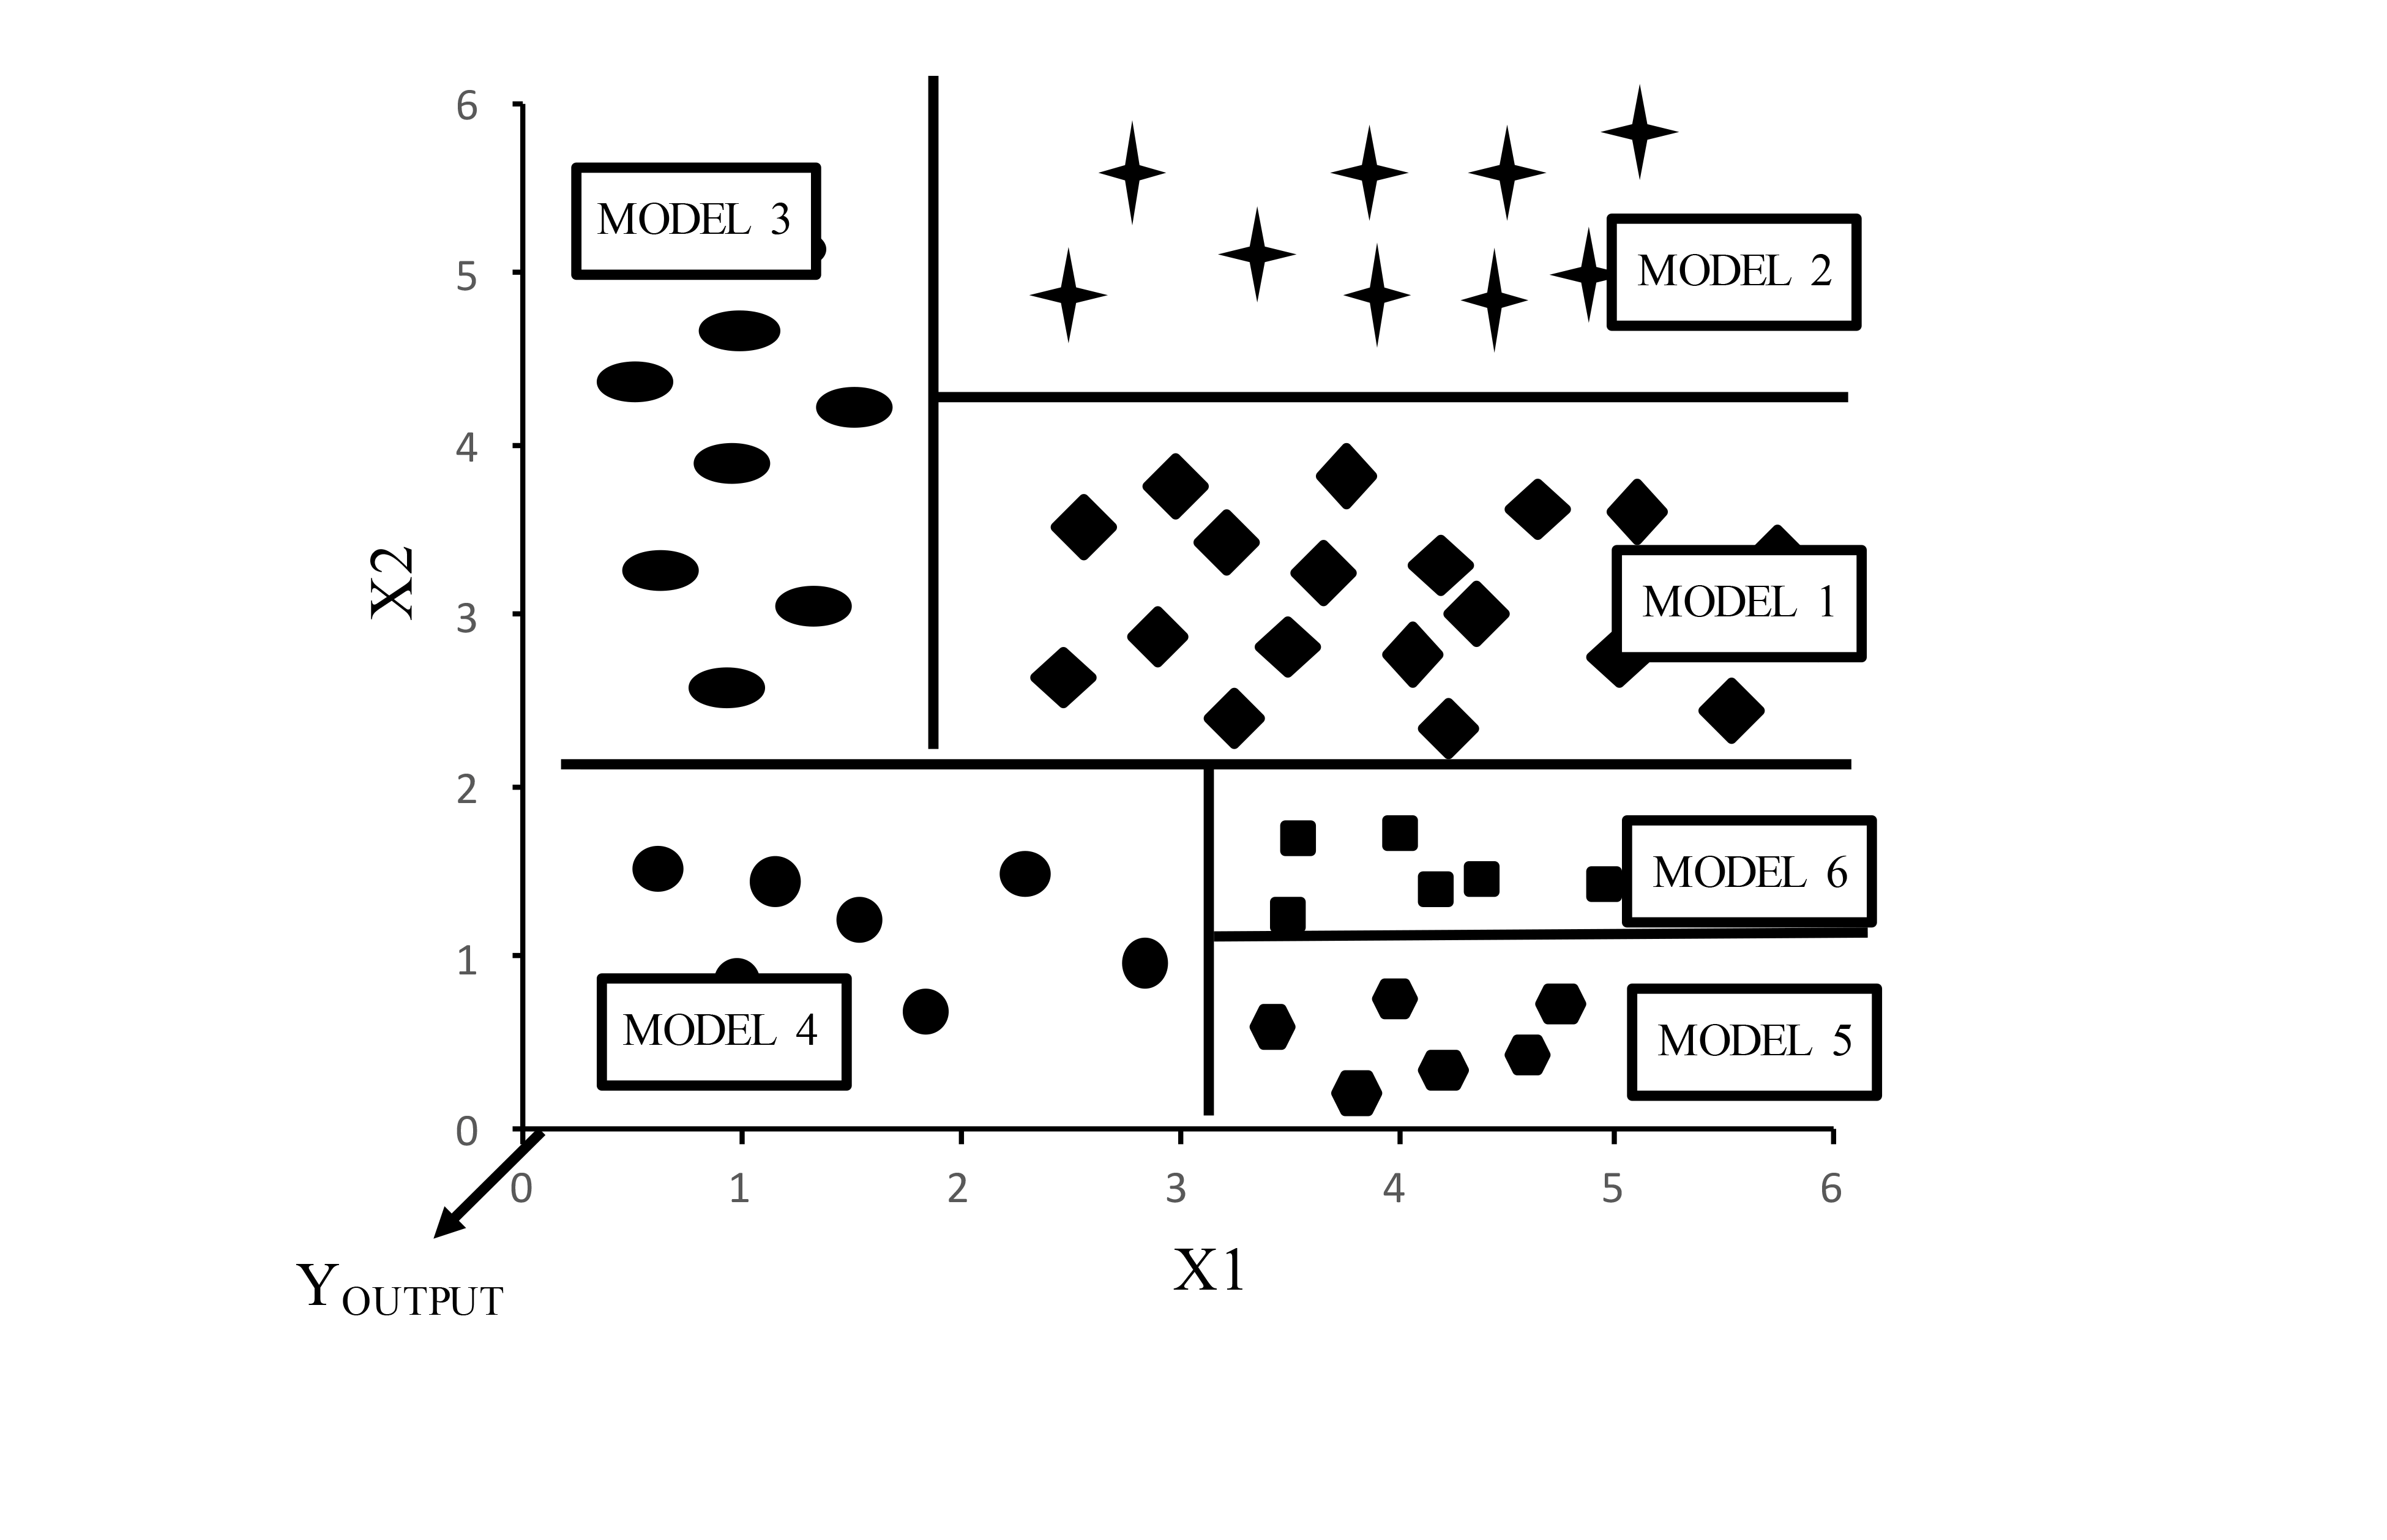
\includegraphics[height=7cm]{splits.png}
\caption{Splitting of the input space (X1 x X2) by M5' model tree algorithm}
\label{fig5}
\end{figure}

\section{Adding another section}
You can show a lot of figures together like these Figures \ref{fig61}, \ref{fig62}, \ref{fig63} below.
\begin{figure} [!htbp]
\centering    
\subfigure[Caption1]{\label{fig61}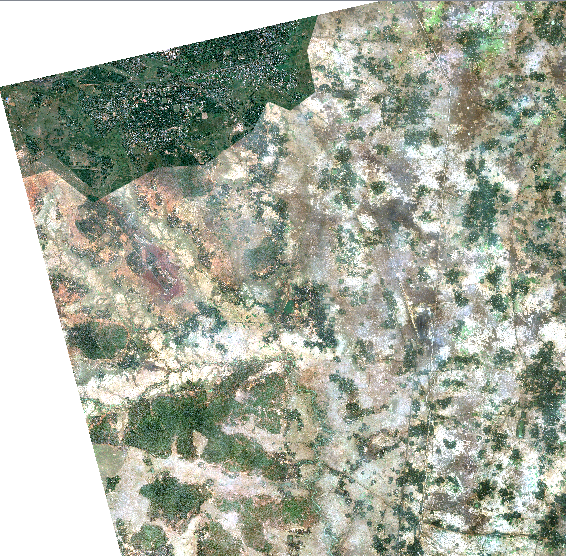
\includegraphics[width=42mm]{data1.png}}
\subfigure[Caption2]{\label{fig62}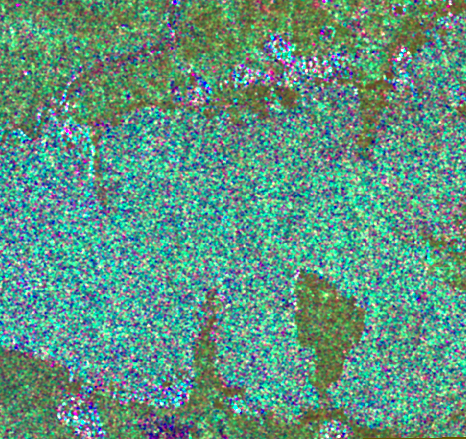
\includegraphics[width=42mm]{data2.png}}
\subfigure[Caption3]{\label{fig63}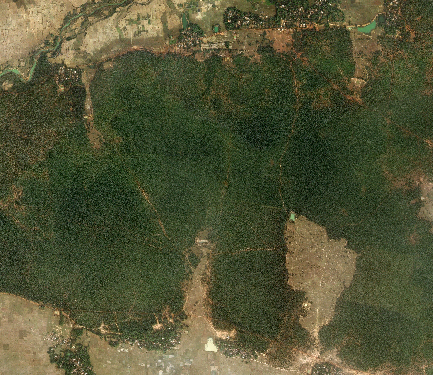
\includegraphics[width=42mm]{data3.png}}
\caption{Figures sample}
\end{figure}
You can add lists into the text like this. 
\begin{itemize}
\settowidth{\leftmargin}{{\Large$\square$}}\advance\leftmargin\labelsep
\itemsep3pt\relax
\renewcommand\labelitemi{{\lower1pt\hbox{\small$\square$}}}
\item	Some sample text item 1. 
\item You may refer to tables \ref{tab1} 
\item Or figures \ref{fig61}
\end{itemize}

Tables can be added like this
\begin{table}[!htbp]
\centering
\caption{Sample table}
\label{tab1}
\begin{tabular}{llll}

\hline
Column 1 & Column 2 & Column 3       \\\hline
1         & Data1 & 13.41179 & 0.9492839 \\
2            & Data2 & 13.39824 & 0.9492952\\\hline
\end{tabular}
\end{table}



%% Chapter Template

\chapter{Result} % Main chapter title

\label{Chapter4} % Change X to a consecutive number; for referencing this chapter elsewhere, use \ref{ChapterX}

\lhead{Chapter 4. \emph{Result}} % Change X to a consecutive number; this is for the header on each page - perhaps a shortened title

%----------------------------------------------------------------------------------------
%	SECTION 1
%----------------------------------------------------------------------------------------

\section{Maximum likelihood Classifier}

Implemented and executed Maximum Likelihood Classifier for stokes parameter with an overall accuracy = 79\%. 

\begin{table}[!htbp]
\centering
\caption{Confusion Matrix for ML Classifier}
\label{tab1}
\begin{tabular}{llll}

\hline
Class  & Forest & Non-Forest & Total Classified pixels      \\\hline
Forest         & 4,129,376 & 1,179,822 & 5,309,198 \\\hline
Non-Forest            & 786,548 & 3,736,102 & 4,522,650 \\\hline
Total ground truth pixels   & 4,915,924 & 4,915,924 & 9,831,848
\end{tabular}
\end{table}

Producer Accuracy for forest class = 83.9\%

Producer Accuracy for non-forest class = 75.9\%

User Accuracy for forest class = 77.7\%

User Accuracy for non-forest class = 82.6\%


%-----------------------------------
%	SUBSECTION 1
%-----------------------------------
\subsection{Discussion}
Upon Visually analyzing the whole image, we can observe that a huge number of pixels that were urban buildup which was not included in the groundtruth.  Figures \ref{fig61}, \ref{fig62}, \ref{fig63} below show a cropped portion of the whole image where forest area can be seen clearly.
\begin{figure} [!htbp]
\centering    
\subfigure[google earth image]{\label{fig61}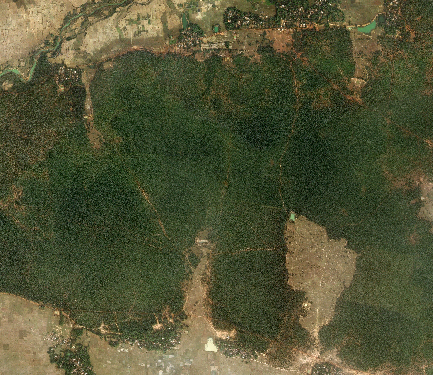
\includegraphics[width=40mm]{data3.png}}
\subfigure[RGB colour composite]{\label{fig62}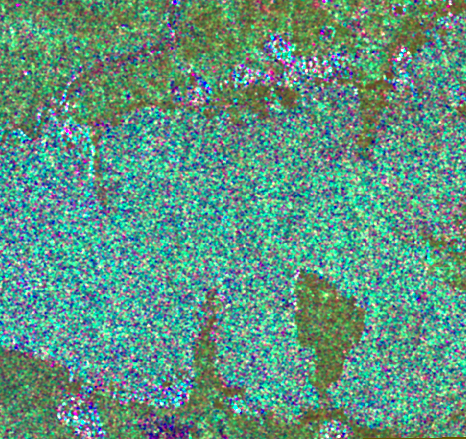
\includegraphics[width=40mm]{data2.png}}
\subfigure[classified image]{\label{fig63}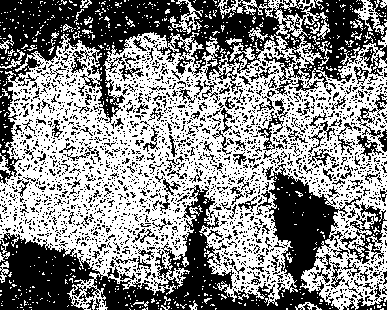
\includegraphics[width=40mm]{data4.png}}
\caption{Figures sample}
\end{figure}
The classifier required additional negative instances as ground truth to actually run and hence introduced difficulty in labelling the same. Maximum Likelihood Classifier used in the QGIS plugin tool assumes that the data pixels are normally distributed, but our data follows a complex distribution other than gaussian and hence did not give a very high accuracy . 
\begin{figure} [!htbp]
\centering    
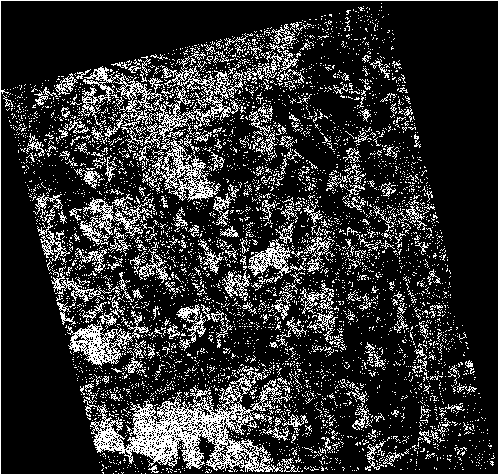
\includegraphics[width=50mm]{data8.png}
\caption{Final output image}
\end{figure}

%----------------------------------------------------------------------------------------
%	SECTION 2
%----------------------------------------------------------------------------------------

\section{One class SVM}

10-fold cross validation was done along with grid search to get the $\nu$ and $\gamma$ parameters and a producer accuracy of 99.08$\%$. for the stokes parameters feature and an accuracy of 98.81$\%$ for m-$\delta$ as feature used for classification.

\begin{table}[!htbp]
\centering
\caption{Parameter values}
\label{tab2}
\begin{tabular}{llll}

\hline
Feature  & $\nu$ & $\gamma$     \\\hline
Stokes parameters   & $9 \times 10^{-4}.$ & $3 \times 10^{-6}.$ \\\hline
m-$\delta$            & $9 \times 10^{-4}.$ & $1 \times 10^{-6}.$ \\\hline
\end{tabular}
\end{table}

%-----------------------------------
%	SUBSECTION 2
%-----------------------------------

\subsection{Discussion}
Even though, we got a good producer accuracy on the given groundtruth, when the classifier was used to predict the whole dataset, visually it was found that a large number of pixels were mispredicted as forest. 
 
%% Chapter Template

\chapter{Conclusion } % Main chapter title

\label{Chapter5} % Change X to a consecutive number; for referencing this chapter elsewhere, use \ref{ChapterX}

\lhead{Chapter 5. \emph{Conclusion}} % Change X to a consecutive number; this is for the header on each page - perhaps a shortened title

%----------------------------------------------------------------------------------------
%	SECTION 1
%----------------------------------------------------------------------------------------

The utilization of features such as Stokes parameter were helpful in detecting forest area in the given dataset. Comparatively, classification with m-$\delta$ values as the feature showed lesser accuracy than when classification is done with stokes parameter as the feature. Maximum Likelihood Classifier requires atleast two classes to work and hence required us to manually label non-forest area, One Class SVM doesn't require negative instances and can hence remove this difficulty. 
%% Chapter Template

\chapter{Future Work} % Main chapter title

\label{Chapter6} % Change X to a consecutive number; for referencing this chapter elsewhere, use \ref{ChapterX}

\lhead{Chapter 6. \emph{Future Work}} % Change X to a consecutive number; this is for the header on each page - perhaps a shortened title

%----------------------------------------------------------------------------------------
%	SECTION 1
%----------------------------------------------------------------------------------------

One class SVM when predicting on the whole dataset visually mispredicted a lot of pixels, this might be due to choosing non-optimal parameters or due to not scaling the data attributes. More optimal parameters can be found. Scaling can improve the accuracy significantly if properly done. Possibility of developing unsupervised classification algorithms based on stokes parameter can be investigated in the future. Image classification methods using Deep Neural Networks in SAR data have surfaced and can be investigated in the future.  
%\input{Chapters/Chapter7} 

%----------------------------------------------------------------------------------------
%	THESIS CONTENT - APPENDICES
%----------------------------------------------------------------------------------------

\addtocontents{toc}{\vspace{2em}} % Add a gap in the Contents, for aesthetics

\appendix % Cue to tell LaTeX that the following 'chapters' are Appendices

% Include the appendices of the thesis as separate files from the Appendices folder
% Uncomment the lines as you write the Appendices

% Appendix Template

\chapter{Appendix A} % Main appendix title

\label{AppendixX} % Change X to a consecutive letter; for referencing this appendix elsewhere, use \ref{AppendixX}

\lhead{Appendix X. \emph{Appendix Title Here}} % Change X to a consecutive letter; this is for the header on each page - perhaps a shortened title

Write your Appendix content here.
%\appendix % Cue to tell LaTeX that the following 'chapters' are Appendices

% Include the appendices of the thesis as separate files from the Appendices folder
% Uncomment the lines as you write the Appendices

%% Appendix Template

\chapter{Appendix A} % Main appendix title

\label{AppendixX} % Change X to a consecutive letter; for referencing this appendix elsewhere, use \ref{AppendixX}

\lhead{Appendix X. \emph{Appendix Title Here}} % Change X to a consecutive letter; this is for the header on each page - perhaps a shortened title

Write your Appendix content here.
%\appendix % Cue to tell LaTeX that the following 'chapters' are Appendices

% Include the appendices of the thesis as separate files from the Appendices folder
% Uncomment the lines as you write the Appendices

%% Appendix Template

\chapter{Appendix A} % Main appendix title

\label{AppendixX} % Change X to a consecutive letter; for referencing this appendix elsewhere, use \ref{AppendixX}

\lhead{Appendix X. \emph{Appendix Title Here}} % Change X to a consecutive letter; this is for the header on each page - perhaps a shortened title

Write your Appendix content here.
%\appendix % Cue to tell LaTeX that the following 'chapters' are Appendices

% Include the appendices of the thesis as separate files from the Appendices folder
% Uncomment the lines as you write the Appendices

%\input{Appendices/AppendixA}
%\input{Appendices/AppendixB}
%\input{Appendices/AppendixC}
%\input{Appendices/AppendixB}
%\input{Appendices/AppendixC}
%\input{Appendices/AppendixB}
%\input{Appendices/AppendixC}
%\input{Appendices/AppendixB}
%\input{Appendices/AppendixC}

\addtocontents{toc}{} % Add a gap in the Contents, for aesthetics

\backmatter

%----------------------------------------------------------------------------------------
%	BIBLIOGRAPHY
%----------------------------------------------------------------------------------------
%\nocite{*}
\label{Bibliography}

\lhead{\emph{Bibliography}} % Change the page header to say "Bibliography"

\bibliographystyle{apalike} % Use the "custom" BibTeX style for formatting the Bibliography

\bibliography{Bibliography} % The references (bibliography) information are stored in the file named "Bibliography.bib"

\end{document}  
